\chapter{Example System 3: Primary/Secondary Pumping}\label{example-system-3-primarysecondary-pumping}

This example will discuss the basics of primary/secondary pumping systems and some of the controls that are used in managing such systems. The input file for this example can be found under the name: PlantApplicationsGuide\_Example3.idf.

Although it is common for these systems to have a common pipe setup to allow for flow imbalance as shown in Figure~\ref{fig:example-of-a-common-pipe-setup} and even though there is a provision in EnergyPlus to model common pipes, this example will not discuss them. In the future, the common pipe is expected to be obsolesced, and therefore using a heat exchanger and two separate loops is recommended for future primary/secondary pumping arrangements.

\begin{figure}[hbtp] % fig 87
\centering
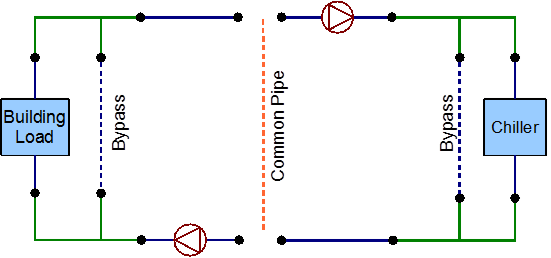
\includegraphics[width=0.9\textwidth, height=0.9\textheight, keepaspectratio=true]{media/image087.png}
\caption{Example of a common pipe setup \protect \label{fig:example-of-a-common-pipe-setup}}
\end{figure}

This system services a three zone building by using, two chillers and purchased cooling on the primary chilled water loop to satisfy the demand loads. The chilled water from the supply side of the primary chilled water loop is passes through a plate heat exchanger which serves as the supply side for the secondary chilled water loop. The cooling coil is placed on the demand side of the secondary loop. The primary loop uses a constant speed pump to circulate the working fluid (water). The secondary loop uses a variable speed pump to manipulate the flow of the fluid such that the cooling coil demand is satisfied. The above mentioned pumps are considered as a primary/secondary pumping pair.

Therefore there are four different loops in the system. The cooling loops in the system will be modeled first. The primary cooling loop (`Primary Chilled Water Loop') which contains a small chiller, a big chiller and a purchased cooling object on the supply side half loop for supplying chilled water to a fluid to fluid plate heat exchanger on the demand side. The secondary cooling loop (`Secondary Chilled Water Loop') contains the fluid to fluid plate heat exchanger on the supply side half loop and a cooling coil on the demand side. The condenser loop (`Condenser Loop') which uses a cooling tower to supply cold water to the chillers on the demand side is modeled next. The heating loop (`Heating Loop') uses purchased heating to serve the demand loads of three reheat coils places in each of the zones of the buildings, this loop will not be discussed in this application guide because it does not relate to the primary/secondary pumping setup in any way.

The plant equipment operation scheme for the primary chilled water loop and the primary/secondary pumping setup are the most important features of this system.

The simple line diagram for the system is shown in Figure~\ref{fig:energyplus-line-diagram-for-the-cooling}. The EnergyPlus line diagram is shown in Figure~\ref{fig:energyplus-line-diagram-for-the-cooling}.

\begin{figure}[hbtp] % fig 88
\centering
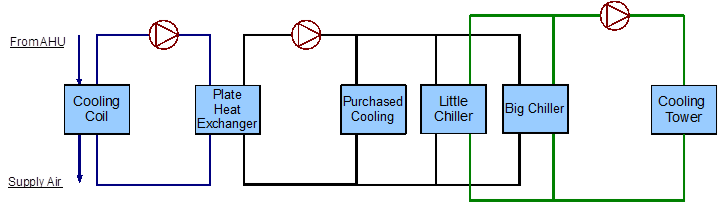
\includegraphics[width=0.9\textwidth, height=0.9\textheight, keepaspectratio=true]{media/image088.png}
\caption{Simple line diagram for the cooling system \protect \label{fig:simple-line-diagram-for-the-cooling-system}}
\end{figure}

\begin{figure}[hbtp] % fig 89
\centering
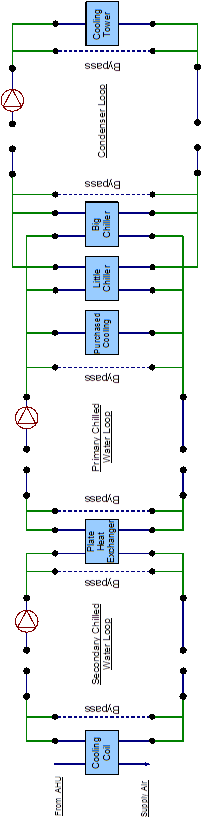
\includegraphics[width=0.9\textwidth, height=0.9\textheight, keepaspectratio=true]{media/image089.png}
\caption{EnergyPlus line diagram for the cooling system \protect \label{fig:energyplus-line-diagram-for-the-cooling}}
\end{figure}
